%%%%%%%%%%%%%%%%%%%%%%%%%%%%%%%%%%%%%%%%%%%%%%%%%%%%%%%%%%%%%%%%%%%%%%%%%%%%%%%%
%2345678901234567890123456789012345678901234567890123456789012345678901234567890
%        1         2         3         4         5         6         7         8

\documentclass[letterpaper, 10 pt, conference]{ieeeconf}  % Comment this line out if you need a4paper

%\documentclass[a4paper, 10pt, conference]{ieeeconf}      % Use this line for a4 paper

%\IEEEoverridecommandlockouts                              % This command is only needed if 
                                                          % you want to use the \thanks command

\overrideIEEEmargins                                      % Needed to meet printer requirements.

% See the \addtolength command later in the file to balance the column lengths
% on the last page of the document

% The following packages can be found on http:\\www.ctan.org
%\usepackage{graphics} % for pdf, bitmapped graphics files
%\usepackage{epsfig} % for postscript graphics files
%\usepackage{mathptmx} % assumes new font selection scheme installed
%\usepackage{times} % assumes new font selection scheme installed
%\usepackage{amsmath} % assumes amsmath package installed
%\usepackage{amssymb}  % assumes amsmath package installed
\usepackage{graphicx} % for pdf, bitmapped graphics files
\usepackage{float}
\usepackage{caption}
\usepackage{subcaption}
%\usepackage{algorithm,algpseudocode}

%\usepackage{epsfig} % for postscript graphics files
%\usepackage{mathptmx} % assumes new font selection scheme installed
%\usepackage{times} % assumes new font selection scheme installed
\usepackage{amsmath} % assumes amsmath package installed
%\usepackage{amssymb}  % assumes amsmath package installed
\usepackage{enumerate}

\title{Project Report:\\\LARGE \bf
Stereo Matching using Graphcut-based Optimization}

\author{Seyed Abbas Sadat\\
Simon Fraser University\\
sas21@sfu.ca% <-this % stops a space
}


\begin{document}



\maketitle
\thispagestyle{empty}
\pagestyle{empty}

%%%%%%%%%%%%%%%%%%%%%%%%%%%%%%%%%%%%%%%%%%%%%%%%%%%%%%%%%%%%%%%%%%%%%%%%%%%%%%%%
\emph{Note: All the figures should be seen on screen in order to distinguish the gray level changes. Also for pixel coordinates $(i,j)$ means row $i$ and column $j$.}


\section{INTRODUCTION}

In this project we developed a stereo matching system based on graph-cut optimization framework \cite{boykov2001fast}. In stereo matching problem, 2 images taken from 2 cameras that are on the same horizontal line are to be matched pixel by pixel. Therefore, for each pixel on the left image, we should find its corresponding pixel on the right image. According to the assumptions, we know that if $(i,j)$ is the coordinate of the pixel in the left image, the coordinate of the corresponding pixel in the right image will be $(i,j-d)$. The unknown variable $d$ is called disparity and is defined in the image space. Disparity is inversely proportional to the depth of the pixel, i.e., the higher the disparity the closer the object. The disparity is not always observable using only 2 images because part of the scene can be occluded in either of the left or right images and hence no matched pixel can be found.

The stereo matching problem is formulated as: given a left and right image, find the most probable disparity image. This \emph{maximum a posteriori} problem is often solved by finding a disparity image that minimizes some energy function. The energy function includes some terms that promote data fidelity (data terms) as well as other terms that support prior assumptions about the solution, e.g., smoothness (smoothness term). These energy functions are non-convex and finding a global optimum it very difficult. Instead, approaches that result in approximation solutions are preferred. One way to reach a local optimum in the minimization is to perform gradient descent. Graph-cuts offer a framework that enables us to generate a movement (step) of current solution that is steepest in terms of minimizing the energy function. By generating and performing these steps iteratively, we reach a local optimum. 

In section \ref{graphcut} we briefly explain how to generate gradient descent moves for a general pixel labelling problem.

\section{Graphcut-based Optimization}
\label{graphcut}
The energy function that we use for stereo matching has the following form:
\begin{figure}[h]
                \centering
                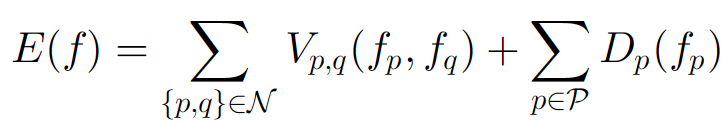
\includegraphics[width=0.35\textwidth]{imgs/energy.png}
                \label{fig:farm}
\end{figure}
\\ \\ \\ \\
Here $D_p(f_p)$ is the data term, i.e. cost of assigning label $f_p$ to pixel $p$. This cost is calculated based on the input data (left and right images in stereo matching). The $V_{p,q}(f_p,f_q)$ term is the pairwise cost of two neighbours $p$, $q$ having labels $f_p$, $f_q$ respectively. 

Assuming that we are at some arbitrary solution we generate an $\alpha\beta-swap$ move or $\alpha-expansion$ move. Next, if performing the new move reduces the energy function, we apply the move on the current solution and generate a new move again iteratively. 

For computing the best move at each solution, i.e. a move with the largest reduction of energy function, we construct a graph network based on the current solution and the input images. The weights of the edges are carefully defined so that the cost of any $cut$ in the created graph equals the cost of the specific move in the labelling problem (plus a constant). Therefore if we find the minimum cut of the graph, we can convert it to a move that reduces the energy function the most.  The following sections describe $\alpha\beta-swap$ and $\alpha-expansion$ moves.

\begin{figure}[h]
                \centering
                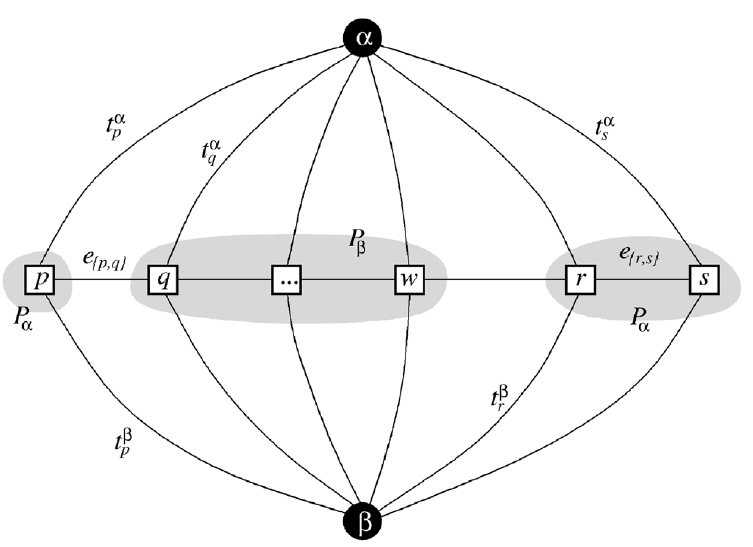
\includegraphics[width=0.5\textwidth]{imgs/swap.png}
                \caption{The graph corresponding to a $\alpha\beta-swap$.}
                \label{abswap}
\end{figure}

\subsection{$\alpha\beta-swap$} 
In $\alpha\beta-swap$ move, subset of the pixel having label $\alpha$ can be changed to label $\beta$ and vice versa. Therefore only the union of the pixel with $\alpha$ or $\beta$ will change labels and other pixel remain the same. Therefore in each cycle of the algorithm this move is computed for each possible label pair and then is applied on the current solution if it reduces the energy function. In order to find the best possible label change in an $\alpha\beta-swap$, the minimum graph-cut problem shown in figure \ref{abswap} is solved:

The terminals are the labels $\alpha$ and $\beta$ and the middle nodes are all the pixels with either $\alpha$ or $\beta$ label. The weight of the terminal edges are the data terms $D_p(\alpha)$ or $D_p(\beta)$, i.e. the cost of assigning the terminal label to the pixel. The weight of the edges between middle nodes are the pairwise smoothness term $V_{p,q}(\alpha,\beta)$. Please see \cite{boykov2001fast} for details.

\subsection{$\alpha-expansion$}
In $\alpha-expansion$ move, a subset of the pixel that do not have label $\alpha$ can be changed to label $\alpha$ and labels of the rest of the pixels remain unchanged. Therefore in each cycle of the algorithm this move is computed for each possible label and then is applied on the current solution if it reduces the energy function. In order to find the best possible label change in an $\alpha-expansion$, the minimum graph-cut problem shown in figure \ref{aexpansion} is solved:

\begin{figure}[h]
                \centering
                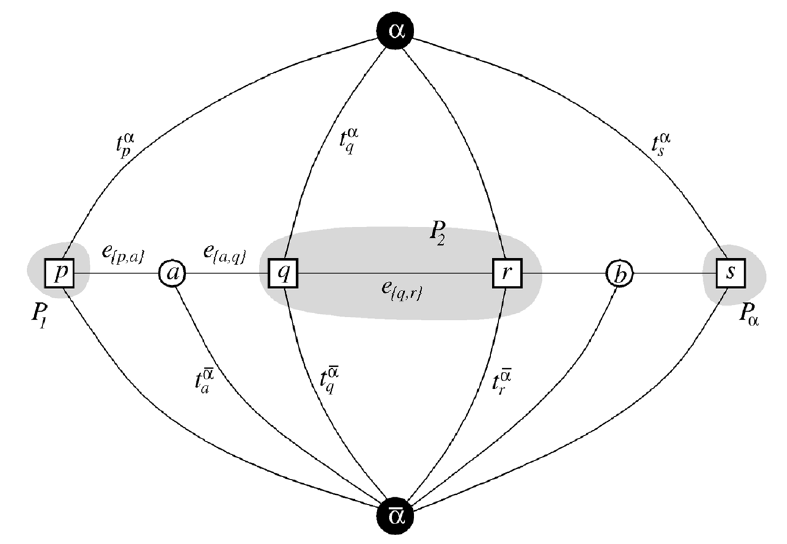
\includegraphics[width=0.5\textwidth]{imgs/expansion.png}
                \caption{The graph corresponding to a $\alpha-expansion$.}
                \label{aexpansion}
\end{figure}

The terminals are the labels $\alpha$ and $\overline{\alpha}$. Selecting $\overline{\alpha}$ simply means that the pixel will keep its current label. The middle nodes are all the pixels with labels other than $\alpha$. The weight of the terminal edges are the data terms $D_p(\alpha)$ or $D_p(f_p)$, i.e. the cost of assigning the terminal label to the pixel. Notice that $D_p(f_p)$ is used when $\overline{\alpha}$ is selected for pixel $p$ and $f_p$ is the current label of pixel $p$. The weight of the edges between middle nodes that with the same labels are the pairwise smoothness term $V_{p,q}(\alpha,f_p)$ in which $f_p$ is the current label of the pair pixels. If the labels of the two neighbour pixels are different we add another axillary node with edges to both corresponding neighbour nodes with weights $V(\alpha,f_p)$ and $V(f_p, \alpha)$ and an edge to the terminal $\overline{\alpha}$ with weight $V(f_q,f_p)$. Please see \cite{boykov2001fast} for details.

\section{Stereo Matching}
As mentioned earlier in stereo matching we want to find the most probable disparity image given the left and right input images. Therefore we minimize an energy function with data terms and smoothness terms involving the disparity labels. More specifically for data term we use the following:
\begin{center}
$D_{i,j}(f)$ $=$ $min\{|I(i,j)-I'(i,j-f)|,200\}$
\end{center}
where $I$ and $I'$ are the left and right image respectively and $f$ is the proposed disparity for pixel $(i,j)$. The constant (200) is to make sure that we are robust to noisy data and outliers. In addition to single pixel cost, we also use window based cost which is the mean of the above data term in a window of size $w$ centred around the corresponding pixel. We will discuss the results in section \ref{exper}.

For the smoothness term we use 2 different models. The first one is the Potts model as follow:
\begin{center}
$V_{p,q}(f_p,f_q)$ $=$ $50*T(f_p \neq f_q)$
\end{center}
This means that if two neighbouring pixel are assigned different disparities, 50 units will be added to the energy function. This model tend to generate large segments with same disparity and is not appropriate for scenes that there is a gradient in depth. We show this in the experiments. For a better smoothness function which preserves linear depth changes we use the following smoothness term: 
\begin{center}
$V_{p,q}(f_p,f_q)$ $=$ $min\{5*|f_p - f_q|,50\}$
\end{center}
This smoothness term penalizes linearly as a function of the disparity difference. We need to cut off these penalties at some point to preserve the edges. We will discuss the results in the next section.
\section{Experiments and Results}
\label{exper}
For the experiments we used the publicly available Middlebury stereo dataset\footnote{http://vision.middlebury.edu/stereo/data/}. Here, we only present the results for 2 different images "Art" in Fig. \ref{art} and "Wood1" in Fig. \ref{wood1}. These figures show the result for pixel level accuracy and subpixel accuracy. By subpixel accuracy we mean that the disparity could have 0.5 disparities. Therfore we can see that the gray level can be different very slightly from the results with pixel level accuracy because of finer resolution.

Next we examine the effect of smoothness model in the energy function. The results are shown in Figure \ref{models}. It can be seen that the Potts model does not allow smooth changes in disparity and large areas with single disparity is preferred. On the other hand, with linear model, a number of disparity changes can be recognized which results in a little smoother disparity image.

We also tested the effect of the size of the window that is used to aggregate the data term. Figure \ref{window} demonstrate the results for 3 different window sizes. We can see that as the window size grows, the changes in disparity becomes smoother. This window act like a low pass filter that removes the high frequencies in the disparity image.

For implementation of this project we used the following libraries:
\begin{itemize}
\item LibCVD\footnote{http://www.edwardrosten.com/cvd/}
\item Min-cut library\footnote{http://vision.csd.uwo.ca/code/}
\end{itemize}
The source code of this project is also publicly available at: $https://github.com/asadat/graphcut\_stereo$.


\begin{figure}
        \centering
        \begin{subfigure}[b]{0.3\textwidth}
                \centering
                
\includegraphics[width=\textwidth]{imgs/l2disparity-expansion-potts.png}
                \caption{The Potts model}
                \label{fig:trees}
        \end{subfigure}%
        
                 %add desired spacing between images, e. g. ~, \quad, \qquad etc.
          %(or a blank line to force the subfigure onto a new line)
        \begin{subfigure}[b]{0.3\textwidth}
                \centering
                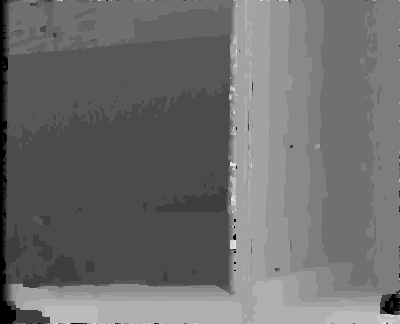
\includegraphics[width=\textwidth]{imgs/l2disparity-expansion-linear.png}
                \caption{Linear model}
                \label{fig:farm}
        \end{subfigure}
        \caption{Disparity image for the "Wood1" dataset using $\alpha$-expansion with Potts and linear smoothness models.}
        \label{models}
\end{figure}

\begin{figure}[t]
        \centering
        \begin{subfigure}[b]{0.3\textwidth}
                \centering
                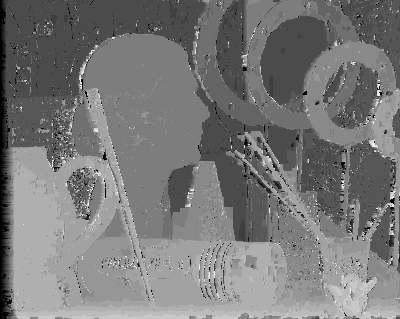
\includegraphics[width=\textwidth]{imgs/l4disparity-expansion-w1.png}
                \caption{$w=1$}
                \label{fig:trees}
        \end{subfigure}%
        
                 %add desired spacing between images, e. g. ~, \quad, \qquad etc.
          %(or a blank line to force the subfigure onto a new line)
        \begin{subfigure}[b]{0.3\textwidth}
                \centering
                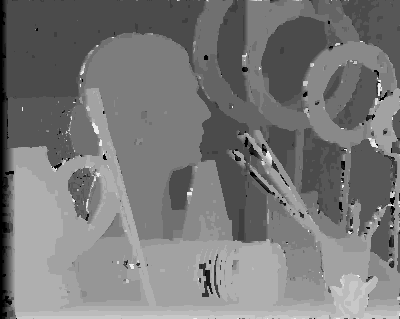
\includegraphics[width=\textwidth]{imgs/l4disparity-expansion-w3.png}
                \caption{$w=3$}
                \label{fig:farm}
        \end{subfigure}
        
                         %add desired spacing between images, e. g. ~, \quad, \qquad etc.
          %(or a blank line to force the subfigure onto a new line)
        \begin{subfigure}[b]{0.3\textwidth}
                \centering
                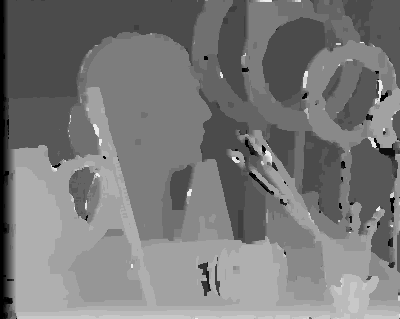
\includegraphics[width=\textwidth]{imgs/l4disparity-expansion-w5.png}
                \caption{$w = 5$}
                \label{fig:farm}
        \end{subfigure}
        \caption{Disparity image for the "Art" dataset using $\alpha$-expansion with 3 different window sizes for data term aggregation.}
        \label{window}
\end{figure}


\begin{figure*}[t]
        \centering
        \begin{subfigure}[b]{0.3\textwidth}
                \centering
                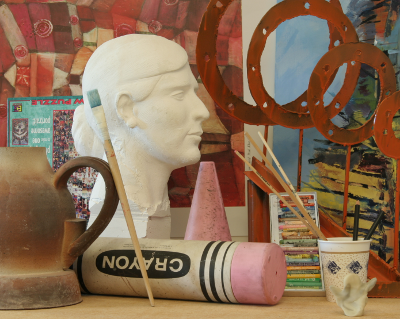
\includegraphics[width=\textwidth]{imgs/l4.png}
                \caption{"Art" Color image}
                \label{fig:trees}
        \end{subfigure}%
                ~ %add desired spacing between images, e. g. ~, \quad, \qquad etc.
          %(or a blank line to force the subfigure onto a new line)
        \begin{subfigure}[b]{0.3\textwidth}
                \centering
                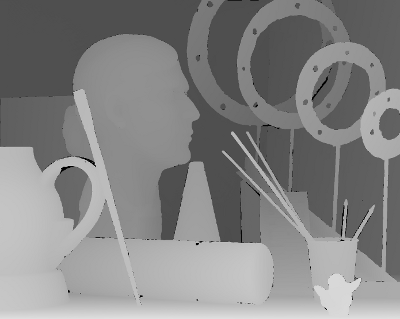
\includegraphics[width=\textwidth]{imgs/disp4.png}
                \caption{Ground Truth}
                \label{fig:farm}
        \end{subfigure}
                ~ %add desired spacing between images, e. g. ~, \quad, \qquad etc.
          %(or a blank line to force the subfigure onto a new line)
        \begin{subfigure}[b]{0.3\textwidth}
                \centering
                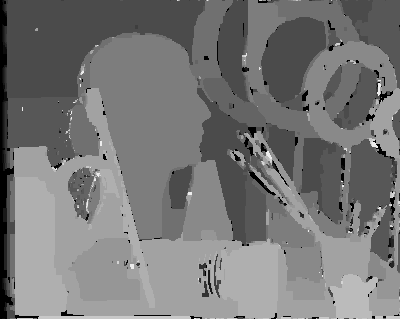
\includegraphics[width=\textwidth]{imgs/l4disparity-expansion.png}
                \caption{$\alpha$-expansion}
                \label{fig:farm}
        \end{subfigure}
                ~ %add desired spacing between images, e. g. ~, \quad, \qquad etc.
          %(or a blank line to force the subfigure onto a new line)
        \begin{subfigure}[b]{0.3\textwidth}
                \centering
                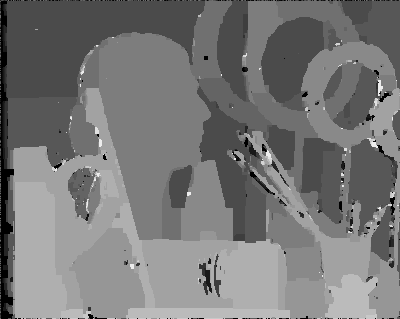
\includegraphics[width=\textwidth]{imgs/l4disparity-swap.png}
                \caption{$\alpha\beta$-swap}
                \label{fig:farm}
        \end{subfigure}
                        ~ %add desired spacing between images, e. g. ~, \quad, \qquad etc.
          %(or a blank line to force the subfigure onto a new line)
        \begin{subfigure}[b]{0.3\textwidth}
                \centering
                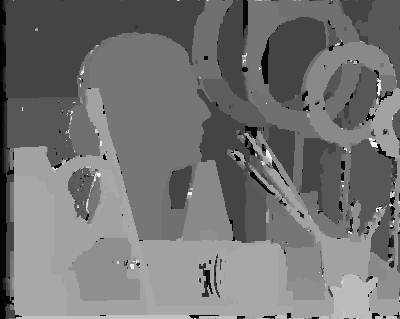
\includegraphics[width=\textwidth]{imgs/l4disparity-expansion-sub.png}
                \caption{$\alpha$-expansion - subpixel accuracy}
                \label{fig:farm}
        \end{subfigure}
                ~ %add desired spacing between images, e. g. ~, \quad, \qquad etc.
          %(or a blank line to force the subfigure onto a new line)
        \begin{subfigure}[b]{0.3\textwidth}
                \centering
                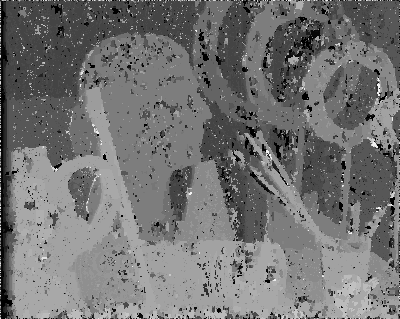
\includegraphics[width=\textwidth]{imgs/l4disparity-swap-sub.png}
                \caption{$\alpha\beta$-swap - subpixel accuracy}
                \label{fig:farm}
        \end{subfigure}
        \caption{Disparity image for the "Art" dataset using the both $\alpha\beta$-swap and $\alpha$-expansion with pixel and subpixel accuracies.}
        \label{art}
\end{figure*}

\begin{figure*}[t]
        \centering
        \begin{subfigure}[b]{0.3\textwidth}
                \centering
                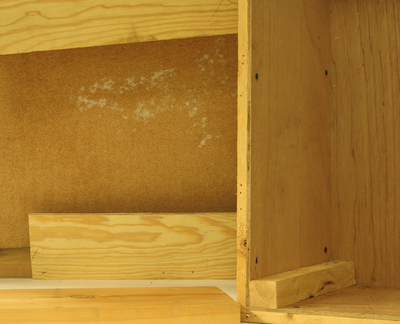
\includegraphics[width=\textwidth]{imgs/l2.png}
                \caption{"Wood1" Color image}
                \label{fig:trees}
        \end{subfigure}%
                ~ %add desired spacing between images, e. g. ~, \quad, \qquad etc.
          %(or a blank line to force the subfigure onto a new line)
        \begin{subfigure}[b]{0.3\textwidth}
                \centering
                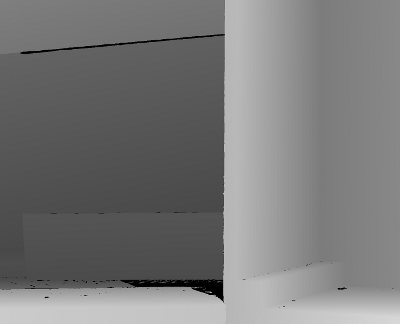
\includegraphics[width=\textwidth]{imgs/disp2.png}
                \caption{Ground Truth}
                \label{fig:farm}
        \end{subfigure}
                ~ %add desired spacing between images, e. g. ~, \quad, \qquad etc.
          %(or a blank line to force the subfigure onto a new line)
        \begin{subfigure}[b]{0.3\textwidth}
                \centering
                
\includegraphics[width=\textwidth]{imgs/l2disparity-expansion.png}
                \caption{$\alpha$-expansion}
                \label{fig:farm}
        \end{subfigure}
                ~ %add desired spacing between images, e. g. ~, \quad, \qquad etc.
          %(or a blank line to force the subfigure onto a new line)
        \begin{subfigure}[b]{0.3\textwidth}
                \centering
                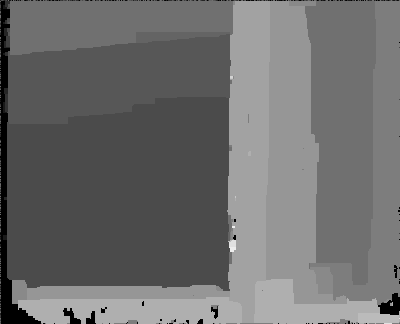
\includegraphics[width=\textwidth]{imgs/l2disparity-swap.png}
                \caption{$\alpha\beta$-swap}
                \label{fig:farm}
        \end{subfigure}
                        ~ %add desired spacing between images, e. g. ~, \quad, \qquad etc.
          %(or a blank line to force the subfigure onto a new line)
        \begin{subfigure}[b]{0.3\textwidth}
                \centering
                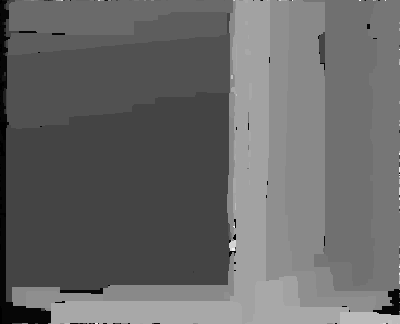
\includegraphics[width=\textwidth]{imgs/l2disparity-expansion-sub.png}
                \caption{$\alpha$-expansion - subpixel accuracy}
                \label{fig:farm}
        \end{subfigure}
                ~ %add desired spacing between images, e. g. ~, \quad, \qquad etc.
          %(or a blank line to force the subfigure onto a new line)
        \begin{subfigure}[b]{0.3\textwidth}
                \centering
                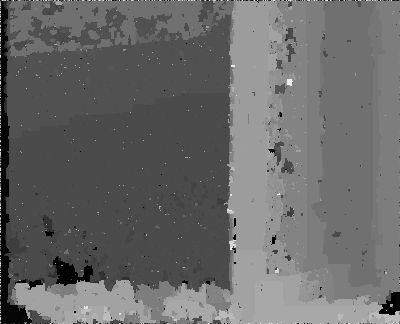
\includegraphics[width=\textwidth]{imgs/l2disparity-swap-sub.png}
                \caption{$\alpha\beta$-swap - subpixel accuracy}
                \label{fig:farm}
        \end{subfigure}
        \caption{Disparity image for the "Wood1" dataset using the both $\alpha\beta$-swap and $\alpha$-expansion with pixel and subpixel accuracies.}
        \label{wood1}
\end{figure*}


\bibliographystyle{ieeetr} 
\bibliography{refs}


\end{document}
